%----------------------------------------------------------------------------------------
%	PACKAGES AND OTHER DOCUMENT CONFIGURATIONS
%----------------------------------------------------------------------------------------
\documentclass[margin, centered]{res}
\topmargin=-0.5in
\oddsidemargin -.5in
\evensidemargin -.5in
\textwidth=6.5in
\itemsep=0in
\parsep=0in
\newsectionwidth{1in}
\usepackage[pdftex]{graphicx}
\usepackage{enumitem}
\usepackage{wrapfig}
\usepackage{helvet}
\usepackage[colorlinks = true,
            linkcolor = black,
            urlcolor  = black,
            citecolor = black,
            anchorcolor = black]{hyperref}
\setlength{\textwidth}{6.5in} % Text width of the document
\setlength{\textheight}{720pt}

\begin{document}

%----------------------------------------------------------------------------------------
%	NAME AND ADDRESS SECTION
%----------------------------------------------------------------------------------------\
\setlength{\voffset}{0.75in}
\begin{center}
    \hspace{-\hoffset}
    \huge\bf{\href{https://www.srm1071.github.io}{SURAJ MANDAL}}
    \hfill 
\smash{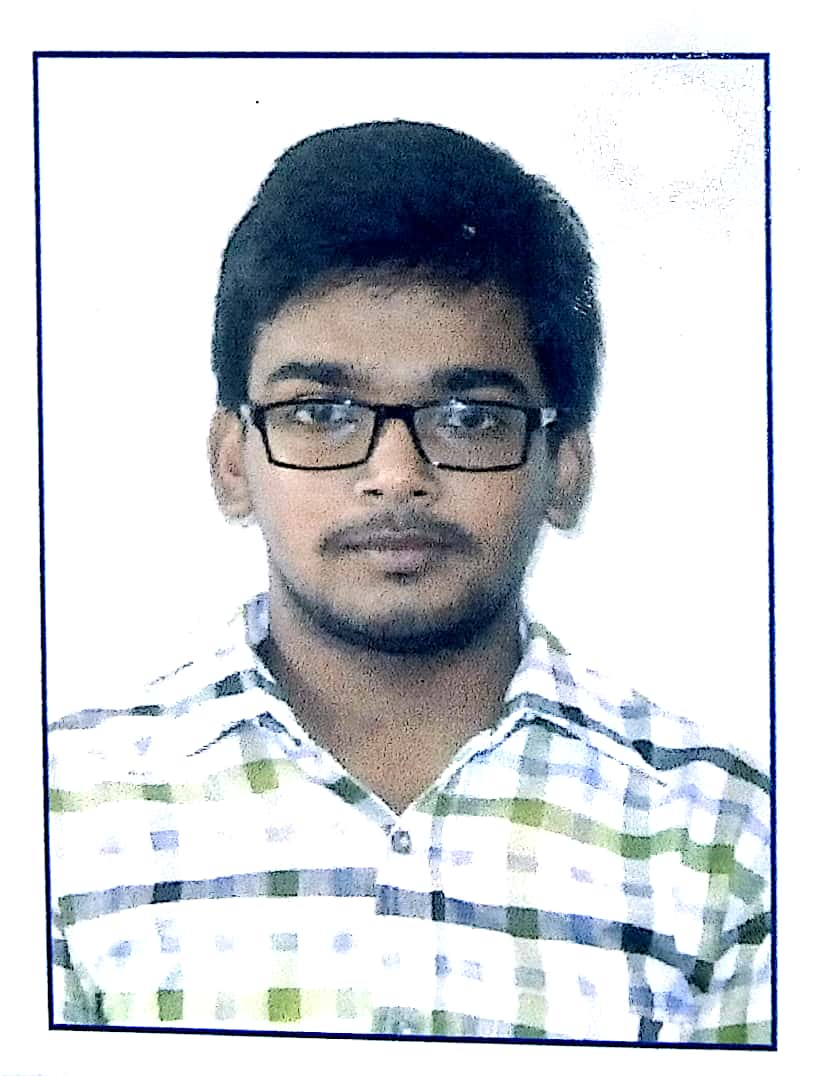
\includegraphics[width=3cm]{suraj.jpg}}
\end{center}
\vspace{-5mm}
\moveleft\hoffset\vbox{\hrule width 19cm height 0.5pt}
\vspace{-7mm}
\begin{center}
    \hspace{-\hoffset}
    \href{mailto:suraj9775@outlook.com}{suraj9775@outlook.com} ~\textbullet~ \(+91\)8513950751 ~\textbullet~ \#Vill: Dangpara, AMARARGARH,BURDWAN, PIN-713144
\end{center}
\vspace{-7mm}
\begin{resume}
\section{Links}
\textbf{Website:} \url{https://srm1071.github.io} \\
\textbf{Github:} \url{https://github.com/srm1071/} \\
\textbf{LinkedIn:} \url{https://www.linkedin.com/in/suraj-mandal-377021128/?ppe=1} \\


%----------------------------------------------------------------------------------------
%	EDUCATION SECTION
%----------------------------------------------------------------------------------------
\section{Education}

\textbf{B.E in Computer Science and Engineering} \hfill 2014-2018 \\
\href{http://http://uit.buruniv.ac.in//}{UNIVERSITY INSTITUTE OF TECHNOLOGY,BURDWAN UNIVERSITY, WEST BENGAL, India}
\begin{itemize}
 \item CGPA of \textbf{Final year student} ()
\end{itemize}
\textbf{High School} -MANKAR HIGH SCHOOL(WBCHSE) - \textbf{63.4\%} \hfill 2011 - 2013 \\
\textbf{Secondary School} - AMARARGARH HIGH SCHOOL(WBBSE) - \textbf{81.75\%} \hfill
 
%----------------------------------------------------------------------------------------
%	WORK EXPERIENCE SECTION
%----------------------------------------------------------------------------------------
\section{Job Experience}
\textbf{fresher}
%----------------------------------------------------------------------------------------
%	OTHER EXPERIENCES SECTION
%----------------------------------------------------------------------------------------

\\
\textbf{Winter Research Intern in DISARM Group, NIT Durgapur} \\
\emph{Mentored by {Dr. Subrata Nandi, Dept. of CSE, NIT Durgapur}} \hfill Dec, 2015 - Jan, 2016 \\
Post-diaster situation analysis and resource management using Delay Tolerant Peer-to-Peer Wireless networks(DISARM).
\\
\\
\textbf{Summer Trainee, {C&IT Department of STEEL
AUTORITY OF INDIA LIMITED, DURGAPUR STEEL PLANT.} \\
\\
\\

%----------------------------------------------------------------------------------------
%	TECHNICAL SKILLS SECTION
%----------------------------------------------------------------------------------------

\section{Technical \hspace{2mm} Skills}
\textbf{Strongest Areas} - Data Structures, Databases, Algorithms, Web Technology \\
\textbf{Languages} - Java, Python, C, C++, UNIX Shell, HTML, CSS. \\
\textbf{Tools} - Git, Android Studio \\
\textbf{Databases} - MySQL \\

%----------------------------------------------------------------------------------------
%	HOBBIES SECTION
%----------------------------------------------------------------------------------------

\section{Hobbies}
Programming,Open source softwares

\section{More}
Please visit \href{https://github.com/srm1071/}{https://srm1071.github.io}

\end{resume}
\end{document}
